\chapter{System Design- Feasibility Study}


The feasibility Study consists primarily of adding a second extruder for PLA materials and an auto-calibration system for the biomaterial extruder.

\section{Conceptual Model}

\begin{figure}[H]
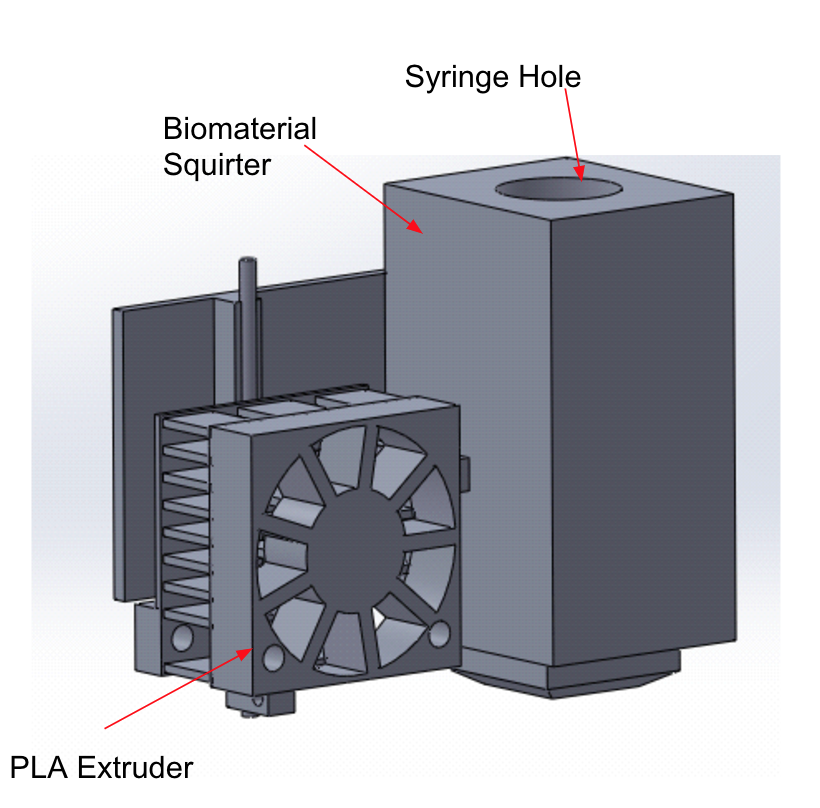
\includegraphics[scale=0.5]{extruder}
\caption{\label{figure:extruder} Rendering of additional PLA extruder module}
\end{figure}

By having a second extruder, the printer can print with both biomaterial and PLA plastic. The module in Figure \ref{figure:extruder} demonstrates how the PLA extruder will be positioned next to the biological extruder. This allows for quick transitions between print materials. 

\begin{figure}[H]
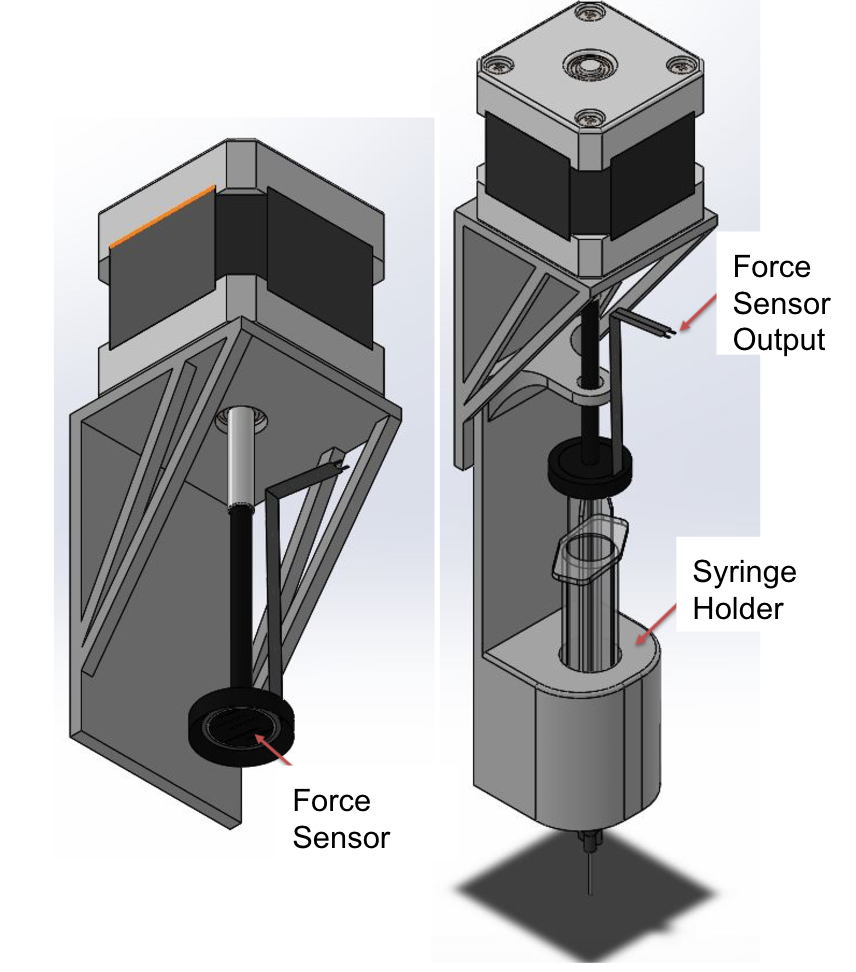
\includegraphics[scale=0.5]{plunger}
\caption{\label{figure:plunger} Rendering of auto-calibration plunger}
\end{figure}

By using a force sensor as shown in Figure \ref{figure:plunger} will be able to detect the amount of force required to drive the plunger. Through testing, we can observe the change in force between various biomaterials and air. Then, we can use the servo motor to drive the plunger until it has been sensed that all of the air has been expelled. 

\section{Technologies Used}
\begin{itemize}
\item Git: A commonly used version control system. Git allows distributed workflow with high data integrity.
\item Arduino Microprocessor: A small, widely used open-source microprocessor commonly used for electronic projects. Arduinos have many controllable input and output pins used to interact with other devices.
\end{itemize}

\section{Design Rationale}

\subsection{Justification for PLA Extruder}
	One of the main features missing from the SE3D printer when compared to other printers in the market is the ability to print with additional materials. By adding a second extruder, the usability of the printer is increased. With the PLA extruder, structural scaffolding can be printed. By using both PLA and biomaterials, more complex structures can be created.

\subsection{Justification for Auto-calibration of Extruder }
	Users of the SE3D printer have given feedback that one of the most difficult aspects for students is proper calibration of the printer. Without proper calibration, prints may fail. By adding auto-calibration to the extruder, we can improve the user experience and decrease the number of failed prints.

\subsection{Justification of Technologies Used}
\begin{itemize}
\item Git: Git was chosen because of its ability to store nearly any type of electronic materials such as images, source code, and documentation. It is commonly used in industry and is well supported. It allows the developers to work concurrently on various parts of the project which results in much faster completion times. Finally, because it is a version control system we can easily reference old code and track changes.

\item Arduino Microprocessor: The Arduino board is commonly used for 3D printers because of its modularity, cheap price, and well supported community. There are many available open-source printer firmwares available that are designed specifically for the Arduino Platform. The Duet board SE3D uses actually switched to Arduino firmware because of the development community around the Arduino Mega. The Arduino can also easily interface with other technologies, such as media readers and LCD screens. Finally, its processor allows for accurate and fast control of stepper motors, which is required for the success of 3D prints.

\end{itemize}
